\documentclass{standalone}
\usepackage{pgfplots}
\pgfplotsset{compat=1.18}

\begin{document}

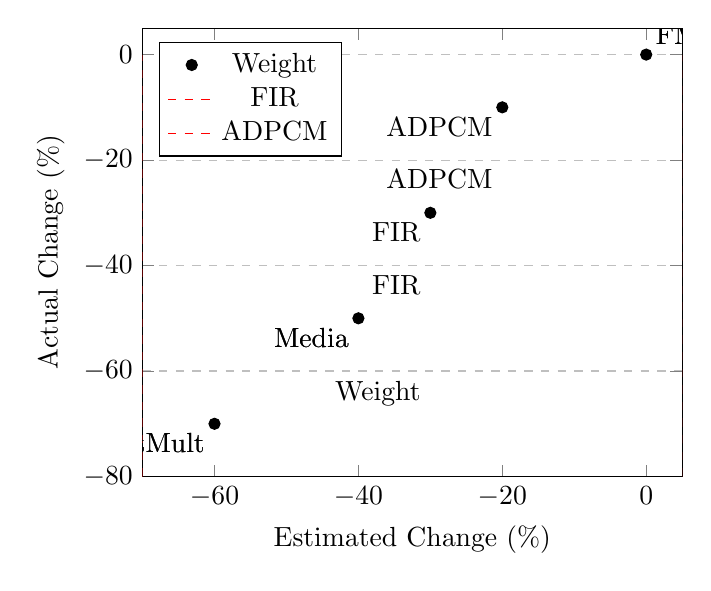
\begin{tikzpicture}
    \begin{axis}[
        xlabel={Estimated Change (\%)},
        ylabel={Actual Change (\%)},
        xmin=-70, xmax=5,
        ymin=-80, ymax=5,
        xtick={-60,-40,-20,0},
        ytick={-80,-60,-40,-20,0},
        legend pos=north west,
        ymajorgrids=true,
        grid style=dashed,
    ]
    
    % Data points
    \addplot[only marks,mark=*] coordinates {
        (-60,-70) [ShiftMult]
        (-40,-50) [Media]
        (-30,-30) [FIR]
        (-20,-10) [ADPCM]
        (0,0) [FMA]
    };
    
    % Red lines representing the synthesis noise window
    \addplot[dashed,red] coordinates {(-70,-80) (-70,0)};
    \addplot[dashed,red] coordinates {(5,-80) (5,0)};
    
    % Labels for data points
    \node at (-60,-70) [anchor=north east] {ShiftMult};
    \node at (-40,-50) [anchor=north east] {Media};
    \node at (-30,-30) [anchor=north east] {FIR};
    \node at (-20,-10) [anchor=north east] {ADPCM};
    \node at (0,0) [anchor=south west] {FMA};
    
    % Legend
    \legend{Weight, FIR, ADPCM, FMA}
    
    % Title and notes
    \node at (axis cs:-30,-60) [anchor=north east] {Weight};
    \node at (axis cs:-30,-40) [anchor=north east] {FIR};
    \node at (axis cs:-20,-20) [anchor=north east] {ADPCM};
    \node at (axis cs:0,0) [anchor=south west] {FMA};
    \node at (axis cs:-60,-70) [anchor=north east] {ShiftMult};
    \node at (axis cs:-40,-50) [anchor=north east] {Media};
    
    \end{axis}
\end{tikzpicture}

\end{document}